%!TEX root = ../DSGEnotes.tex
\chapter{似然估计}
\label{sec:mle-model}

\section{线性模型}
\label{sec:linear-model}

设一组含有$n$个观察数据的随机变量$\left\{ y_{i} \right\}, \, i = 1,\ldots,n$。假定其中每个观察符合正态分布$y_{i} \sim \mathcal{N} \left( \mu_{i}, \sigma^{2} \right)$。由设定可见,对于$i,j \in [1,n], \, i \neq j$,均值也许不同,但方差相同。

正态分布(normal distribution)\index{normal distribution! \dotfill 正态分布}又称高斯分布(Gaussian distribution)\index{Gaussian distribution \dotfill 高斯分布},如$y_{i}$的概率密度方程(probability density function, PDF)\index{probability density function (PDF) \dotfill 概率密度方程} $f\left( y_{i} \right)$定义为
\begin{equation}
  \label{eq:mle-pdf-def}
  f \left( y_{i} \right) = \frac{1}{\sqrt{2 \pi \sigma^{2}}}
  \exp \left[
  - \frac{1}{2} \frac{
  \left( y_{i} - \mu_{i} \right)^{2}
  }{
  \sigma^{2}
  }
   \right],
\end{equation}
均值为$0$方差为$1$的高斯分布,见图\ref{fig:mle-pdf}所示。

\begin{lstlisting}[language=R]
# 正态分布的概率密度方程(均值=0,方差=1)
x <- seq(-4,4,length=100)
hx <- dnorm(x)
plot(hx ~ x, type="l", lty = 1, col="blue",
     xlab="y", ylab="Density",
     main = "Probability Density Function (normal distribution)")
\end{lstlisting}

\begin{figure}[htbp]
  \caption{正态分布的概率密度方程}
  \centering
  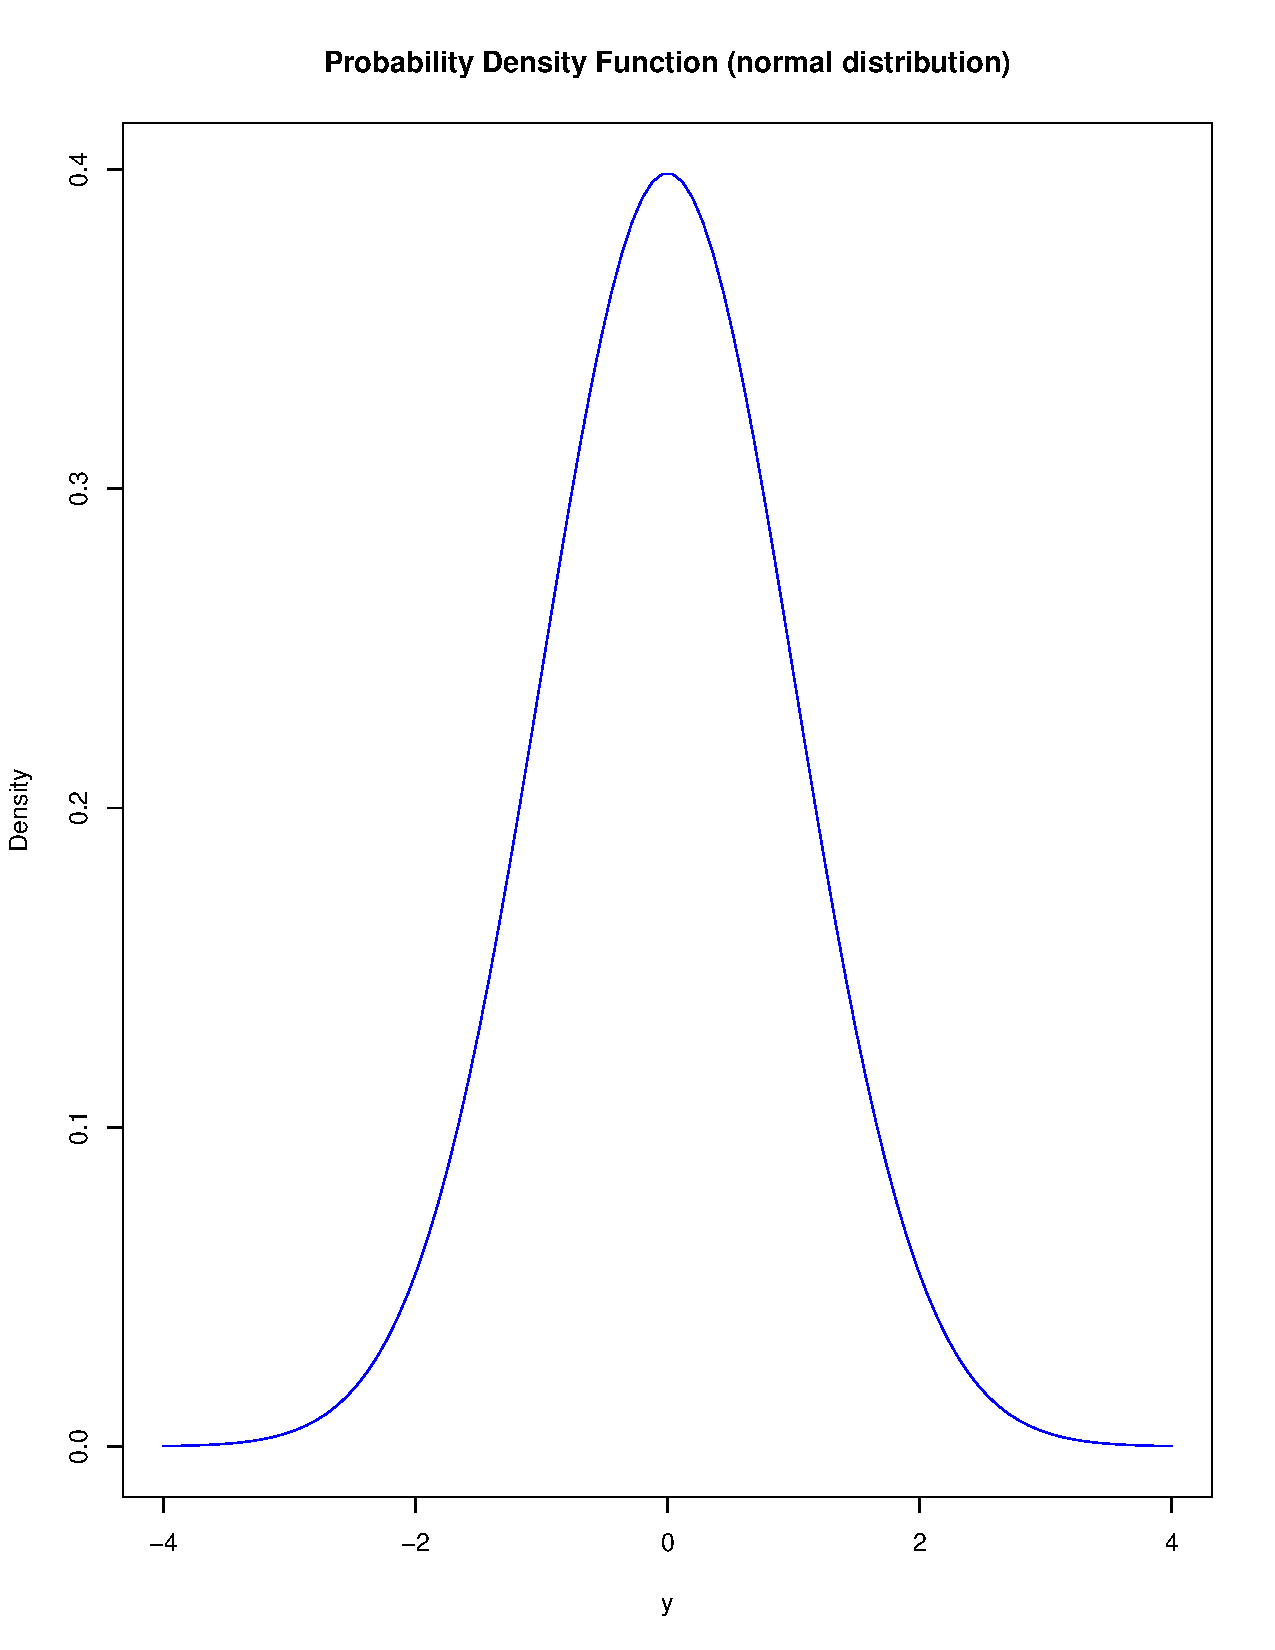
\includegraphics[width=8cm]{./Figures/20180421-pdf-function}
  \label{fig:mle-pdf}
%
%  \small{Source: PBOC.}
\end{figure}

现在引入额外的假定,对于全部$i, j \in [0,n], \, i \neq j$,设观测数据$y_{i}$和$y_{j}$相互独(mutually independent),即$\cov \left( y_{i}, y_{j} \right) = 0$。这使得我们能够计算观测数据集中全部数据的联合分布(joint distribution),即$\prod_{i=1}^{n} f \left( y_{i} \right)$,进而勾勒出似然方程,用于进一步的估计和检测。

把$\left\{y_{i}\right\}_{i=1}^{n}$表示为一个$(n \times 1)$的列向量$Y$,对应均值$E Y = \mu$,方差协方差矩阵$\var(Y) = \sigma^{2} I$,其中$I$是单位矩阵。列向量$\mu = \left\{ \mu_{i} \right\}_{i=1}^{n}$。
由于$n$个观测变量$y_{i}$彼此不相关且方差相同,$\var(Y)$满足以下特征:对角元素全是$\sigma^{2}$,非对角元素全是$0$。进而$Y$呈多元正态分布(multivariate normal distribution)\index{normal distribution!multivariate \dotfill 多元正态分布}
\begin{equation}
  \label{eq:multivariate-normal-distribution}
  Y \sim \mathcal{N}_{n} \left( \mu, \sigma^{2} I \right).
\end{equation}

来看\eqref{eq:multivariate-normal-distribution}的模型。假定$Y = y_{1}, y_{2}, \ldots, y_{n}$与某组预测变量$X = x_{1}, x_{2}, \ldots, x_{n}$有关,进一步说,第$i$个观测变量$y_{i}$的期望值$\mu_{i}$,与$x_{i1}, x_{i2}, \ldots, x_{ip}$有关,呈线性关系,满足
\begin{equation}
  \label{eq:mle-linear-relationship-yx-np}
  \mu_{i} = \beta_{1} x_{i1} + \beta_{2} x_{i2} + \ldots + \beta_{p} x_{ip} \Longleftrightarrow \mu_{i} = x_{i}^{\top} \beta,
\end{equation}
其中$x_{i}^{\top}$是由$p$个预测变量$x_{i1}, x_{i2}, \ldots ,x_{ip}$组成的行向量。待求解的未知系数$\beta = \beta_{1}, \ldots, \beta_{p}$称回归系数。将全部$n$个\eqref{eq:mle-linear-relationship-yx-np}加总可得
\begin{equation}
  \label{eq:mle-linear-relationship-mu-x-beta}
  \underset{\left( n \times 1 \right)}{\mu} =
  \underset{\left( n \times p \right)}{X}
  \underset{\left( p \times 1 \right)}{\beta},
\end{equation}
我们常将解释变量的矩阵$X$称为模型矩阵(model matrix)\index{model matrix \dotfill 模型矩阵}或设计矩阵(design matrix)\index{design matrix \dotfill 设计矩阵}。对应地,$X \beta$称线性预测子(linear predictor)。

最简单的线性模型可以假定每个观测数据的期望值都相同$\mu_{i} = \mu \, \forall \, i$,称零模型(null model)\index{null model \dotfill 零模型}。另一个极端是$\mu_{i} \neq \mu_{j} \, \forall \, i \neq j$,称饱和模型(saturated model)\index{saturated model \dotfill 饱和模型},此时观测数据量$n$越大,待估计的线性系数$\beta$数量就越多($p \times n$)。

零模型和饱和模型是两个极端。现实应用中常取折中,致力于分析导致线性预测子$X \beta$产生结构差异的系统性原因,进而分析观测数据$y$和均值$\mu$之间的非结构性差异(或称随机差异),用误差项来表示。

\section{参数估计}
\label{sec:mle-parameter-estimation}
来看模型$\mu_{i} = x_{i}^{\top} \beta$。问题:如何估计参数$\beta, \sigma^{2}$?

\subsection{回归系数的估计}
\label{sec:mle-estimation-beta}
我们的求解思路是,建立似然方程(likelihood function, LHF)\index{likelihood function (LHF)\dotfill 似然方程},选取使(对数)似然方程最大化的参数值。如果观测数据之间互相独立,那么LHF是一组正态PDF \eqref{eq:mle-pdf-def}的乘积
\begin{equation}
  \label{eq:mle-lhf-pdf-product}
  \log L \left( \beta, \sigma^{2} \right) = - \frac{n}{2} \log \left( 2 \pi \sigma^{2} \right) - \frac{1}{2} \sum_{i=1}^{n}
  \frac{
  \left( y_{i} - \mu_{i} \right)
  }{
  \sigma^{2}
  },
\end{equation}
$\mu_{i}$如\eqref{eq:mle-linear-relationship-yx-np}所定义。RHS中可定义残差平方和(residual sum of squares, RSS)\index{residual sum of squares (RSS) \dotfill 残差平方和}
\begin{equation}
  \label{eq:mle-rss-def}
  RSS (\beta) = \sum_{i=1}^{n} \left( y_{i} - \mu_{i} \right)^{2}
  = \left( y - X \beta \right)^{\top} \left( y - X \beta \right).
\end{equation}

不难看出,在给定$\sigma^{2}$值不变的情况下,最佳系数$\hat{\beta}$的选取符合
\begin{equation}
  \label{eq:mle-lhf-argmax-beta}
  \hat{\beta} =\underset{\beta}{\argmax} \log L \left( \beta, \sigma^{2} \right)
  = \underset{\beta}{\argmin} \frac{\rss(\beta)}{\sigma^{2}},
\end{equation}
也即,我们的目标是选取合适的$\beta = \hat{\beta}$,使对应的模拟值$\mu_{i}$尽可能接近实际观测值$y_{i}$。

求解$\argmin \rss (\beta)$等价于求解$\rss \left( \hat{\beta} \right) =0$,即
\begin{equation*}
  y - X \hat{\beta} = 0 \quad \Rightarrow y = X \hat{\beta} \quad \Rightarrow X^{\top} y = X^{\top} X \hat{\beta}
\end{equation*}
如果模型矩阵$X$列满秩,那么$X^{\top} X$也是满秩的,因而$X^{\top} X$可逆。由此可得线性系数$\hat{\beta}$的OLS估计式(同时也是MLE估计式)
\begin{equation}
  \label{eq:mle-argmin-beta-hat-estimation}
  \hat{\beta} = \left( X^{\top} X \right) X^{\top} y.
\end{equation}
我们将这个方程称为正规方程(normal equation)\index{normal equation \dotfill 正规方程}。

反之,如果$X$不是列满秩的,可以计算$\left( X^{\top} X \right)^{\dagger}$,称为伪逆矩阵(第\ref{sec:simple-pseudo}节)。但比起这种相对复杂的计算来,还是直接删除$X$中的冗余列更加方便。当前大多数主流统计软件都足够只能,可以自动识别并删除冗余列。

求解正规方程\eqref{eq:mle-argmin-beta-hat-estimation}需要借助数值方法。数值方法有多种,常见的如
\begin{itemize}
  \item 从$\left( X^{\top} X \right)$入手,方法如高斯消元法(第\ref{sec:numlin-gaussian-elimination}节)、Cholesky分解(第\ref{sec:numlin-factorization-cholesky}节)等。
  \item 对模型矩阵$X$做因子分解,如
  \begin{itemize}
    \item Householder reflections
    \item Givens rotations
    \item Gram-Schmidt正交(第\ref{sec:orthogonality-polynomials}节),等
  \end{itemize}
\end{itemize}
结合大多数主流数值计算软件,可以执行上述数值运算。

基于\eqref{eq:mle-lhf-argmax-beta},利用最小化RSS方法测得的系数$\hat{\beta}$,是一个不依赖于$\sigma^{2}$的值——方差值是事先给定的。因此我们称$\hat{\beta}$为最大似然法的全局最大解(global maximum)。

对于零模型的情况:$X$是一组$1$构成的向量;$\left( X^{\top} X \right) = n$和$X^{\top} y = \sum_{i=1}^{n} y_{i}$是两个标量;$\hat{\beta} = \bar{y}$是样本的均值。这就是说,计算出的样本均值,可堪称是在线性模型中做最大似然估计的一个最简单的例子。

关于MLE $\hat{\beta}$,有以下几个有趣的性质。

\begin{enumerate}
\item BLUE
\begin{enumerate}
  \item 如果模型设定正确,即从(弱的)意义上说,给定$x_{i}$的情况下,观测$y_{i}$的期望值$\mu_{i}$就等于$x_{i}^{\top} \beta$,此时的OLS估计$\hat{\beta}$是个无偏估计(unbiased estimator),OLS 估计$\hat{\beta}$的期望值就等于真实参数值$\beta$
\begin{equation}
  \label{eq:mle-hat-beta-unbiased}
  E \hat{\beta} = \beta.
\end{equation}
  \item 如果观测数据之间彼此不相关$\cov \left(y_{i}, y_{j} \right) = 0, \, \forall \, i \neq j$,并且同方差$\sigma_{i}^{2} = \sigma_{j}^{2}= \sigma^{2}$。那么,一方面根据\eqref{eq:mle-rss-def}-\eqref{eq:mle-lhf-argmax-beta},$\hat{\beta}$是一个关于$y$的线性方程,另一方面根据假定,观测数据集合$Y$的方差协方差矩阵$\var(Y) = \sigma^{2} I$,那么OLS估计$\hat{\beta}$的方差协方差矩阵为
  \begin{equation}
    \label{eq:mle-hat-beta-varcov}
    \var \left( \hat{\beta} \right) = \left( X^{\top} X \right)^{-1} \sigma^{2},
  \end{equation}
  因此,基于观测数据,构建线性方程模型所做的全部无偏OLS估计$\left\{\beta\right\}$中,MLE估计$\hat{\beta}$是最佳线性无偏估计(best linear unbiased estimator, BLUE)\index{best linear unbiased estimator (BLUE) \dotfill 最佳线性无偏估计}。对于某一给定的观测样本,由于再没有其他无偏估计的方差会低于$\var \left( \hat{\beta} \right)$,我们称OLS估计$\hat{\beta}$是有效估计(efficient estomator)\index{efficient estimator \dotfill 有效估计}。
\end{enumerate}

\item OLS估计$\hat{\beta}$在大样本观测集合中的抽样分布,接近于多元正态分布,其均值和方差如\eqref{eq:multivariate-normal-distribution}所定义,满足
\begin{equation*}
  \hat{\beta} \sim \mathcal{N}_{p} \left( \beta, \left(X^{\top}, X \right)^{-1} \sigma^{2} \right).
\end{equation*}

\item 将前两个性质代入零模型,可见样本均值$\bar{y}$是对$\mu$的无偏估计;$\bar{y}$的方差为$\frac{\sigma^{2}}{n}$,在大样本下近似正态分布。

\item 前三条性质的生成,依赖于对观测数据的均值、方差协方差的最高到二阶矩条件的假设,包括
\begin{equation*}
  E Y = X \beta, \quad \var \left( Y \right) = \sigma^{2} I.
\end{equation*}

\item 基于观测数据的联合正态分布假定,所测得的OLS估计$\hat{\beta}$也是MLE。如果$Y \sim \mathcal{N}_{p} \left( X \beta, \sigma^{2} I \right)$,那么$\hat{\beta}$的样本分布恰好也是多元正态分布,对应的、方差也是
\begin{equation*}
  \hat{\beta} \sim \mathcal{N}_{p} \left( \beta, \left(X^{\top}, X \right)^{-1} \sigma^{2} \right).
\end{equation*}.
\end{enumerate}

需要指出的是,上属性质虽然重要,但不应被过分夸大:只有在小样本数据的统计推断中,才需要假定观测数据是正态分布的。而真正重要的假设其实是观测数据之间彼此不相关,同方差:这些对于大样本数据下的统计推断至关重要。

\subsection{方差的估计}
\label{sec:mle-estimation-variance}
将求得的OLS估计$\hat{\beta}$ \eqref{eq:mle-argmin-beta-hat-estimation}代回log LHF \eqref{eq:mle-lhf-pdf-product},可得一个关于方差$\sigma^{2}$的最大(对数)似然方程,又称描述似然方程(profile likelihood function)\index{profile likelihood function \dotfill 描述似然方程}
\begin{equation}
  \label{eq:mle-estimation-variance-plhe}
  \log L \left( \sigma^{2} \right)
  = - \frac{n}{2} \log \left( 2 \pi \sigma^{2} \right)
  - \frac{1}{2} \frac{
  \rss \left( \hat{\beta} \right)
  }{\sigma^{2}}.
\end{equation}

类似地,$\hat{\sigma}^{2} = \underset{\sigma^{2}}{\argmin} \partial \log L \left( \sigma^{2} \right)$,等价于求解$\underset{\sigma^{2}}{\arg} \left[ \frac{\partial \log L \left( \sigma^{2} \right)}{\partial \sigma^{2}} = 0 \right]$,求得的值为方差的MLE
\begin{equation*}
  \hat{\sigma}^{2} = \frac{\rss \left( \hat{\beta} \right)}{n},
\end{equation*}
需要指出的是,$\hat{\sigma}^{2}$是有偏估计;我们可以将分母用$n-p$代替$n$来变为无偏估计(类似于在估计方差时用$n0-1$代替$n$)。

在零模型中,方差$\sigma^{2}$的估计是样本方差:这是由于$\hat{\beta} = \bar{y}, \, \rss = \sum_{i=1}^{n} \left( y_{i} - \bar{y} \right)$。在正态分布的假定条件下,比值$\left( \frac{\rss }{\sigma^{2}}\right)$呈$\chi^{2}$分布(DoF n-p),并且与线性系数估计值$\hat{\beta}$无关。

小提示:使用$\chi^{2}$分布作为LHF来估计$\sigma^{2}$,比起使用高斯分步来同时估计$\beta, \sigma^{2}$来,会得到无偏估计。

\section{假设检验}
\label{sec:mle-hypothesis-testing}
如何对回归系数向量估计$\hat{\beta}$作假设检验?具体来说,这个问题可以分为两种情况
\begin{itemize}
  \item 对向量$\beta$中的某个系数$\beta_{i}$作显著程度检验,
  \item 对几个、甚至全部系数作显著程度检验,
\end{itemize}
本节介绍一些常见的检测方法,尤其是
\begin{itemize}
  \item 基于MLE的抽样分布的Wald检验,
  \item 似然率检验。
\end{itemize}

\subsection{Wald检验}
\label{sec:mle-wald-test}
假设我们只检测系数向量$\beta$中某一系数$\beta_{j}$的显著性,如
\begin{equation*}
  H_{0}: \beta_{j} = 0,
\end{equation*}
如果零假设成立,那么其MLE $\hat{\beta}_{j}$的分布情况因此可写为$\sim \mathcal{N} \left( 0, \var \left( \hat{\beta}_{j} \right)  \right)$,
其中方差 $\var \left( \hat{\beta}_{j} \right) $是方差协方差矩阵
$\var \left( \hat{\beta} \right)$
\eqref{eq:mle-hat-beta-varcov}中第$j$个对角元素的值。那么可以考虑如下比值,定义为Wald 统计量$t$
\begin{equation}
  \label{eq:mle-wald-t-def}
  t_{j} = \frac{\hat{\beta}_{j}}{\sqrt{\var \left( \hat{\beta}_{j} \right)}},
\end{equation}
计算$t_{j}$的难度在于,\eqref{eq:mle-hat-beta-varcov}中全体方差$\sigma^{2}$常常未知。在实际应用中,常常将$\sigma^{2}$替换为无偏估计$\hat{\sigma}^{2}$
\begin{equation}
  \label{eq:mle-wald-hat-var}
  \hat{\sigma}^{2} = \frac{\rss \left(\hat{\beta}\right)}{n-p}.
\end{equation}

假设观测数据符合正态分布,$\hat{\sigma}^{2}$依照\eqref{eq:mle-wald-hat-var}计算,那么在零假设下$\hat{\sigma}^{2}$呈学生$t$分布(student's t distribution),DoF n-p。

具体来说,若观测数据的二阶弱假设条件(均值、方差、方差协方差)得到满足,那么$t$值 \eqref{eq:mle-wald-t-def}在大样本下近似为标准正态分布。这为大样本数据下的近似推断打下良好基础。

一些研究中,不考虑数据样本量的大小,直接将\eqref{eq:mle-wald-t-def}作为学生$t$统计,而且这值得进一步讨论。
\begin{enumerate}
  \item 若样本量大,假定条件``观测数据是否符合正态分布"的确不重要;
  \item 若样本量相对较小,那么正态分布的假定是否成立,对Wald检测是否有效会产生决定性影响。
  对于规模适中的观测样本,应当审慎使用$t$检测:Student's t值随着自由度趋近于无穷大而收敛至标准正态分布\footnote{如双边95$\%$的关键$t$值是2.09 (20 DoF),1.98 (100 DoF),而标准正态分布的关键$t$值是1.96 (100 DoF)。}。
\end{enumerate}

$t$值可用于描述一个系数估计的置信区间(confidence interval)\index{confidence interval \dotfill 置信区间},例如,某个真实系数值$\beta_{j}$以$100 \times \left( 1 - \alpha \right) \%$的置信率落在统计区间中
\begin{equation}
  \label{eq:mle-wald-confidence-interval}
  \hat{\beta}_{j} \pm t_{
  \frac{1-\alpha}{2}, n-p
  }
  \sqrt{\var \left( \hat{\beta}_{j} \right)}.
\end{equation}
其中$t_{
\frac{1-\alpha}{2}, n-p
}$表示$n-p$ DoF,$\alpha$样本大小的学生$t$双边分布的关键值。

Wald检验也可用于检测一组系数的联合置信区间。将系数向量$\beta$分解为两块
\begin{equation*}
  \underset{\left\{ 1 \times p \right\}}{\beta^{\top}} =
  \left(
  \underset{\left\{ 1 \times p_{1} \right\}}{\beta_{1}^{\top}},
  \underset{\left\{ 1 \times p_{2} \right\}}{\beta_{2}^{\top}}
  \right),
\end{equation*}

建立零假设
\begin{equation*}
  H_{0}:\beta_{2} = 0.
\end{equation*}

在求得MLE $\hat{\beta}$后,将Wald检验统计量表示为二次形式
\begin{equation}
  \label{eq:mle-wald-joint-statistic}
  W =
  \hat{\beta}_{2}^{\top}
  \left( \var \left( \hat{\beta}_{2} \right) \right)^{-1}
  \hat{\beta}_{2},
\end{equation}
如前所述,我们用$\frac{ \var \left( \hat{\beta} \right)}{n-p}$近似替代全$\sigma^{2}$,用于测算方差协方差矩阵$\var \left( \hat{\beta}_{2} \right)$。若$p_{2}=1$即$\beta_{2}$只有一个系数,那么\eqref{eq:mle-wald-joint-statistic}回复到
\eqref{eq:mle-wald-hat-var}的形式。

根据渐进理论(asymptotic theory),在零假设$H_{0}$下,大样本MLE $\hat{\beta}_{2}$符合多元正态分布,均值向量为$0$,方差协方差矩阵为$\var \left( \hat{\beta}_{2} \right)$。由此可得,二次形Wald统计$W$ \eqref{eq:mle-wald-joint-statistic}在大样本下也是一个$\chi^{2}$分布,对应$p_{2}$ DoF。无论$\sigma^{2}$是实现给定的值,还是利用$\rss$作近似估计,上述结论都成立。

如果我们持有更强形式的假定,即观测数据呈正态分布,那么检验的结果也是更强形式的。此时若$\sigma^{2}$值事先给定,$W$就恰好是$\chi^{2}$分布($p_{2}$ DoF)。若用$\frac{\rss \left( \hat{\beta} \right)}{n-p}$来近似估计$\sigma^{2}$ (对应$p_{2}$ DoF),则$\frac{W}{p_{2}}$呈一个对应于$p_{2}$和DoF $n-p$ 的$F$分布。

值得注意的是,给定$p$值不变,随着$n \rightarrow \infty$,$ \left( n-p \right) \rightarrow \infty$,$F_{p_{2}, n-p} \times p_{2} \rightarrow \chi^{2} \, \left( p_{2} \, DoF \right)$。这意味着在大样本情况下,将$W$统计量视作$\chi^{2}$分布,或是将$W/p_{2}$视作$F$分布,二者并无本质区别。

\subsection{似然率检验}
\label{sec:mle-lhr-test}
还来看多系数联合显著水平检验的例子,对应零假设
\begin{equation*}
  H_{0}:\beta_{2} =0.
\end{equation*}

我们可以将模型矩阵$X$相应地分解为
\begin{equation*}
  \underset{\left\{p \times 1 \right\}}{X} = \left(
  \underset{\left\{p_{1} \times 1 \right\}}{X_{1}},
  \underset{\left\{p_{2} \times 1 \right\}}{X_{2}}
  \right),
\end{equation*}
如果零假设成立,这意味着后面的$p_{2}$个解释变量$X_{2}$对观测数据$Y$无影响。

可以建立似然率检验(likelihood ratio test, LHR)指标,
对零假设做检验,分两步走
\begin{enumerate}
  \item 分别构建两个嵌入模型并作拟合。
  \begin{enumerate}
    \item 小模型:只考虑前$p_{1}$个解释变量$X_{1}$。
    \item 大模型:用全部$p = p_{1} + p_{2}$ 个解释变量$X$。
  \end{enumerate}
  \item 比较两个模型的最大(对数)似然方程。
\end{enumerate}

先来看只考虑$X_{1}$的小模型。基于给定的方差$\sigma^{2}$,对应似然方程\eqref{eq:mle-lhf-pdf-product},可得最大似然方程
\begin{equation}
  \label{eq:mle-mlh-small-model}
  \max \log L \left( \beta_{1} \right) = c - \frac{1}{2} \frac{\rss \left( X_{1} \right)}{\sigma^{2}}, \quad c = - \frac{n}{2} \log \left( 2 \pi \sigma^{2} \right),
\end{equation}
其中常数$c$的值取决于$n$和$\sigma^{2}$。

对应地,考虑$X = \left(X_{1}, X_{2} \right)$的大模型,最大似然方程
\begin{equation}
  \label{eq:mle-mlh-big-model}
  \max \log L \left( \beta_{1}, \beta_{2} \right)
  = c - \frac{1}{2} \frac{\rss \left( X_{1} + X_{2} \right)}{\sigma^{2}}.
\end{equation}

将两个最大似然方程\eqref{eq:mle-mlh-small-model},\eqref{eq:mle-mlh-big-model}相减,定义为$\log \lambda$,作为似然率量(likelihood ratio criterion, LHRC)\index{likelihood ratio criterion (LHRC) \dotfill 似然率量}
\begin{equation}
  \label{eq:mle-mlh-lhrc}
  - 2 \log \lambda = \max \log L \left( \beta_{1} \right) - \max \log L \left( X_{1}, X_{2} \right) = \frac{
  \rss \left( X_{1} \right) - \rss \left( X_{1} + X_{2} \right)
  }{
  \sigma^{2}
  }.
\end{equation}

关于LHRC,有两点说明
\begin{enumerate}
  \item 通过两个最大似然方程的差值,该指标反映在引入额外的$p_{2}$个解释变量$X_{2}$后,$\rss$的变化情况。通常来说,如果$\Delta \rss >0$,那么$X_{2}$对观测数据可能是有显著影响的。
  \item 对$\Delta \rss$除以方差$\sigma^{2}$是作单位标准化处理,表示残差平方和的变化是以总方差的单位计。如果这个比值(最大似然率)超过了事先预期值,就表示$X_{2}$的确是显著的,零假设不成立。
\end{enumerate}

这就涉及到如何设定``事先预期”值,它与样本的分布有关。根据大样本定律可知,随着$n \rightarrow \infty$,样本分布逐渐收敛至$\chi^{2}$ ($p_{2}$ DoF)。对于$\chi^{2}$分布,已知期望值和方差分别为$\nu$和$2 \nu$,那么事先预期的设定可以使:每增加额外$1$个变量$p_{2} \rightarrow p_{2} + 1$,会导致$\Delta \rss$减少$\sigma^{2}$个单位,对应标准化后的单位$1$。具体说来,若$\rss$的下降幅度超过$95\%$百分位(percentile)的参考分布值,就表示为误差的缩减超出预期。

类似地,LHRC \eqref{eq:mle-mlh-lhrc}的计算难度在于$\sigma^{2}$可能未知。可以用用大模型$\rss \left( X_{1} + X_{2} \right)$的方差估计$\hat{\sigma}^{2}$作近似替代,计算方法为
\begin{equation*}
  \hat{\sigma}^{2} = \frac{
  \rss \left( X_{1} + X_{2} \right)
  }{n-p},
\end{equation*}
代回\eqref{eq:mle-mlh-lhrc},算得的大样本下LHRC分布依旧是$\chi^{2}$分布($p_{2}$ DoF)。

若观测样本符合正态分布这一更强假定,结果也相应更强。如果$\sigma^{2}$是已知的,那么LHRC $- 2 \log \lambda$就恰好是$\chi^{2}$分布($p_{2}$ DoF)。如果$\sigma^{2}$未知,是用估计出的$\hat{\sigma}^{2}$作近似替代,那么对应的LHRC除以$p_{2}$,即$\frac{- 2 \log \lambda}{n-p}$就恰好是一个$F_{p_{2}, n-p}$分布,满足
\begin{equation}
  \label{eq:mle-mlh-lhrc-f}
  F = \frac{
  \frac{1}{p_{2}}
  \left[
  \rss \left( X_{1} \right) - \rss \left( X_{1} + X_{2} \right)
  \right]
  }{
  \frac{1}{n-p} \rss \left( X_{1} + X_{2} \right)
  },
\end{equation}
分子表示在每一单位自由度减少,导致$\rss$的减少幅度;分母是平均$\rss$,反映模型总体的噪声情况。通常来说,如果测得的$F$统计值高于$F$分布在$95\%$下对应$p_{2}, \, n-p$的关键值,那么我们可以拒绝零假设$H_{0}$,$X_{2}$的确对观测数据产生影响。

\subsection{Anova表}
\label{sec:mle-anova}
在实际应用中,到底应该用基于大样本分布下最大似然估计的Wald检验,还是基于最大(对数)似然估计比较的似然率检验呢?答案是,随着$n$值逐渐增大,两种检测方法渐进等价。若模型是线性的,则回答更为明确:两种检测完全等价。详细证明过程略,我们可以在一些具体应用中涉及相关讨论。

值得指出的是,两种检验的(渐进)等价基于模型的线性结构假定。对于非线性模型如logistic模型、泊松回归模型等,两种检测是有区别的。通常说来,对线性模型的检测而言,我们可以提出以下建议:
\begin{itemize}
  \item 对单个系数可用Wald检验 \eqref{eq:mle-wald-t-def},
  \item 多个系数的检验,或者进一步对多个嵌入模型的比较,可用LHRC的$F$检验 \eqref{eq:mle-mlh-lhrc-f}。
\end{itemize}

测算$F$统计所需的计算,常收录在anova表中(analysis of variance table, anova)\index{analysis of variance table (anova) \dotfill anova表}。表格将整体$\rss$分为三个部分,小模型$X_{1}$的$\rss$、加入$X_{2}$后大模型的$\rss$、剩余$\rss$。每个$\rss$项后还附有DoF,以及平均值$\frac{\rss}{DoF}$,如表所示。

\begin{table}[h]
\caption{anova表}
\begin{center}
\begin{threeparttable}
\begin{tabular}{c c c}
    \toprule
     & $\rss$ & DoF \\ \midrule
      QWERTY\tnote{1}   &                     &                       \\
      ASDFGH\tnote{2}   &                     &                       \\ \bottomrule
\end{tabular}
\begin{tablenotes}
\item[1] qwerty; \item[2] asdfgh
\end{tablenotes}
\end{threeparttable}
\end{center}
\label{table:simDisimCoefNewDef}
\end{table}
